\section{Perfomance Metrics for Image Classification}
Evaluating the performance of a Machine learning model is one of the important steps while building an effective ML model. To evaluate the performance or quality of the model, different metrics are used, and these metrics are known as performance metrics or evaluation metrics. These performance metrics help us understand how well our model has performed for the given data. In this way, we can improve the model's performance by tuning the hyper-parameters. Each ML model aims to generalize well on unseen/new data, and performance metrics help determine how well the model generalizes on the new dataset\cite{c-eval}.
\par \vspace{1em}
In a classification problem, the category or classes of data is identified based on training data. The model learns from the given dataset and then classifies the new data into classes or groups based on the training. It predicts class labels as the output, such as Yes or No, 0 or 1, Spam or Not Spam, etc. \par \vspace{1em}

To evaluate the performance of a classification model, different metrics are used, and some of them are as follows:

    \subsection{Accuracy}
    The accuracy metric is one of the simplest Classification metrics to implement, and it can be determined as the number of correct predictions to the total number of predictions.

    \begin{center}
        \(\displaystyle{Accuracy = \frac{\text{No Of Correct Prediction}}{\text{Total Number Of Prediction}}}\) 
    \end{center}


    \subsection{Confusion Matrix}
    A confusion matrix is a tabular representation of prediction outcomes of any binary classifier, which is used to describe the performance of the classification model on a set of test data when true values are known.

    \begin{figure}
        \centering
        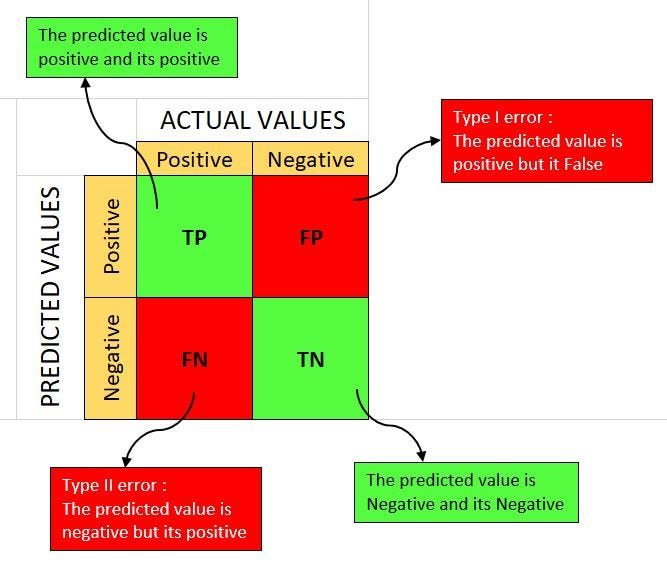
\includegraphics[width=0.75\linewidth]{graphics//chapter3/typical confusion matrix.png}
        \caption{Confusion Matrix, Source: \cite{WEBSITE:cm-credit}}
        \label{fig:typical-confusion-matrix}
    \end{figure}

    In general, the confusion matrix table is divided into four terminologies, which are as follows:
    \begin{enumerate}
        \item \textbf{True Positive(TP):} In this case, the prediction outcome is true, and it is true in reality, also.
        \item \textbf{True Negative(TN):} in this case, the prediction outcome is false, and it is false in reality, also.
        \item \textbf{False Positive(FP):} In this case, prediction outcomes are true, but they are false in actuality.
        \item \textbf{False Negative(FN):} In this case, predictions are false, and they are true in actuality.
    \end{enumerate}



    
    \subsection{Precision}    
    Precision (also called positive predictive value) gives the proportion of positive identifications that were actually correct. Written as a formula\cite{precision-recall}:
    \begin{center}
        \(\displaystyle{\text{Precision} = \frac{\text{TP}}{\text{TP + FP}}}\) 
    \end{center}
    
    
    
    \subsection{Recall}
    It is also similar to the Precision metric, however, it aims to calculate the proportion of actual positives that was identified incorrectly. It can be calculated as True Positive or prediction that are actually true to the total number of positives, either correctly predicted as positive or incorrectly predicted as negative (true Positive and false negative)\cite{precision-recall}.
    \begin{center}
        \(\displaystyle{\text{Recall} = \frac{\text{TP}}{\text{TP + FN}}}\) 
    \end{center}

    \subsection{When to use Precision and Recall}

    \begin{figure}
        \centering
        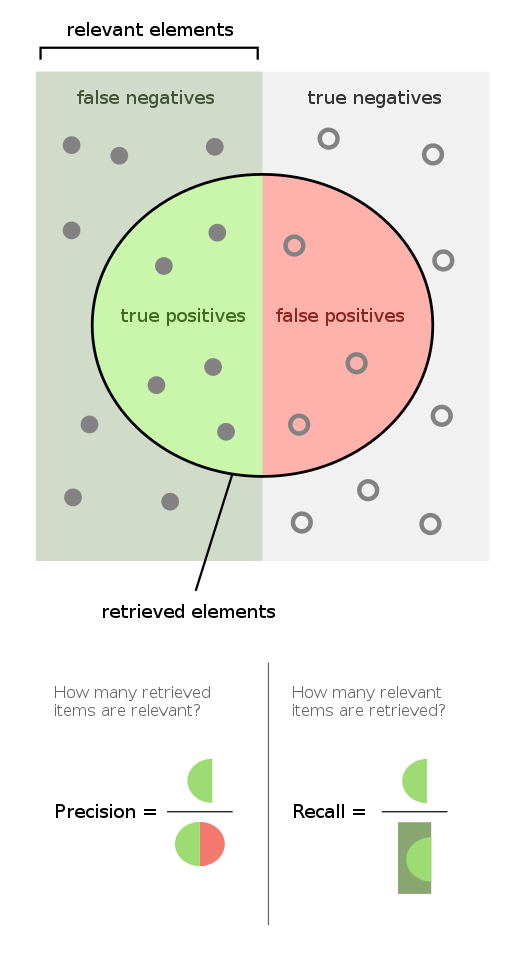
\includegraphics[width=0.5\linewidth]{graphics//chapter3/Precisionrecall.svg.png}
        \caption{Precision and Recall}
        \label{fig:precision-recall}
    \end{figure}
    From the above definitions of Precision and Recall, we can say that recall determines the performance of a classifier with respect to a false negative, whereas precision gives information about the performance of a classifier with respect to a false positive.\par\vspace{1em}
    So, if we want to minimize the false negative, then, Recall should be as near to 100\%, and if we want to minimize the false positive, then precision should be close to 100\% as possible.In simple words, if we maximize precision, it will minimize the FP errors, and if we maximize recall, it will minimize the FN error.
    
    \subsection{F1 Score}
    F-score or F1 Score is a metric to evaluate a binary classification model on the basis of predictions that are made for the positive class. It is calculated with the help of Precision and Recall. It is a type of single score that represents both Precision and Recall. So, the F1 Score can be calculated as the harmonic mean of both precision and Recall, assigning equal weight to each of them.\par \vspace{1em}

    The formula for calculating the f1 score is given below\cite{c-eval}: 
    \begin{center}
        \(\displaystyle{\text{F1 Score} = 2 * \frac{\text{precision} * \text{recall}}{\text{precision} + \text{recall}}}\) 
    \end{center}

    \subsection{When to use F-Score}
    As F-score make use of both precision and recall, so it should be used if both of them are important for evaluation, but one (precision or recall) is slightly more important to consider than the other. For example, when False negatives are comparatively more important than false positives, or vice versa.\\par \vspace{1em}
    
    % \subsection{Importance Precision vs Recall Trade-off }
    % Both precision and recall may be useful in cases where there is imbalanced data. However, it may be valuable to prioritize one over the other in cases where the outcome of a false positive or false negative is costly. For example, in medical diagnosis, a false positive test can lead to unnecessary treatment and expenses. In this situation, it is useful to value precision over recall. In other cases, the cost of a false negative is high. For instance, the cost of a false negative in fraud detection is high, as failing to detect a fraudulent transaction can result in significant financial loss.\par\vspace{1em}
    
    % \textbf{Trade-off Scenarios}
    % \begin{enumerate}
    %     \item \textbf{High Precision, Low Recall:} This scenario is favorable in situations where false positives are costly. For instance, in spam detection, high precision ensures that non-spam emails are rarely misclassified as spam.
    %     \item \textbf{High Recall, Low Precision:} This scenario is preferable when missing a positive case is more detrimental. In medical diagnosis, high recall ensures that most patients with the disease are correctly identified, even if some healthy individuals are incorrectly flagged.
    % \end{enumerate}
    % Balancing precision and recall is crucial for applications requiring a compromise between the two, such as fraud detection or information retrieval systems.


    % \subsection{F1-Score as a Balanced Metric}
    % The F1-Score provides a single metric that balances precision and recall, particularly useful when the class distribution is imbalanced.\par\vspace{1em}
    % The F1-Score is the harmonic mean of precision and recall, emphasizing that both metrics are equally important. Unlike the arithmetic mean, the harmonic mean penalizes extreme values more, ensuring that both precision and recall need to be sufficiently high to achieve a high F1-Score.\par\vspace{1em}

    % \textbf{Benefits of F1-Score}
    % \begin{itemize}
    %     \item Balanced Evaluation: It balances the importance of both false positives and false negatives.
    %     \item Imbalanced Datasets: It is particularly useful for imbalanced datasets where accuracy might be misleading.
    %     \item Unified Metric: It provides a single, interpretable metric to evaluate the model's performance.
    % \end{itemize}
